\chapter{Battery SOC Estimation Algorithms}\label{ch:Battery_SOC_Estimation_Algorithms}
We require high-power storage batteries to meet the energy needs of multiple systems. The Lithium-ion batteries are the most popular varieties. Due to their safety, electrochemical structure, high number of charge/discharge cycles, high voltage, and high energy density, they are the most ideal rechargeable battery technologies. This battery type requires a particular charge technique called Constant Current- Constant Voltage (CC-CV) \cite{Coulomb_Counting_SOC_Estimation}.

\section{Coulomb Counting Algorithm (CC)}

State of Charge (SoC) is the most crucial characteristic to keep an eye on to prevent overcharging and deep drain, which can harm the battery's internal structure and even hurt safety.
For estimating the SoC of the lithium-ion battery, several methodologies have been put out in the literature. Both direct and indirect techniques are included in this category. The Coulomb Counting (CC) approach, which takes into account an initial value of SoC (SoC0), and updates it by integrating the current over the nominal capacity, is one example of a direct method that we notice. The CC algorithm has some drawbacks, and the Enhanced CC (ECC) fixes those drawbacks. Using information extracted from the SoC-OCV curve, the open circuit voltage (OCV) estimation is performed.

There are several strategies for indirect methods that can be divided into model-based methods, such as electrical and electrochemical models, and adaptive models, such as the Kalman filter, neural network, or fuzzy logic.
For the model-based ones, certain techniques need for the characterization of the model parameters from a fresh battery, which is expensive and time-consuming. Some of these techniques also can't be used online and call for an understanding of the battery's chemical composition. Due to their great complexity, adaptive models struggle with battery model efficiency and require a significant amount of data training.

The ratio of the nominal capacity to the current capacity is known as the SoC. The CC approach involves taking into account a starting SoC0 value and then updating it by integrating the current over time.
The CC approach has some inefficiencies. In actuality, the SoC0 value is not predetermined, and this method does not take into account the aging factor that influences the Qnom value or the self-discharge phenomenon after extended storage. An ECC approach is suggested as a solution to these problems.
To determine the SoC0 value at each cycle and subsequently update the $100\%$ SoC value, this algorithm takes into account the self-discharging losses and presents a recalibration method for battery propriety at a fully charged state and an empty state.

\begin{equation}\label{eq:batt_SOC_def}
    SOC = \frac{Q_{act}}{Q_{nom}}
\end{equation}

\begin{equation}\label{eq:batt_SOC_CC}
    SOC = SOC_0 + \int_{t_0}^{t_0 + dt} \frac{i_{batt}}{Q_{nom}} 
\end{equation}
\section{Kalman Filter}\label{sec:KalamanFilter}
In essence, a Kalman filter is a system of recursive equations that implements a predictor-corrector type estimator. It creates an ideal guess of the system state based on the input control and output measurements; as a result, it is typically employed when the system state cannot be directly monitored and needs to be predicted optimally from the output measurements \cite{SOC_Estimation_KalmanFilter_Ahmad}.
In this section \ref{sec:KalamanFilter}, the extended Kalman filter (EKF) for non-linear systems is explained, followed by the discrete Kalman filter for linear systems, and lastly a state space model for the Li-Ion battery is built up. To assess the reliability of the suggested method, comparisons are also made between SOC values calculated by Ampere-counting and SOC values estimated by EKF \cite{SOC_Estimation_KalmanFilter_Liu}.

\subsection{The Discrete Kalam Filter}\label{sec:Discrete_Kalam_Filter}
This section outlines the fundamental design of a Kalman filter, which takes measurements and estimates the system state at discrete time intervals \cite{LIPO_Batt_Parameters_identification_Rahmoun}.

The linear difference stochastic equation \ref{eq:Discrete_State_Equation} governs a discrete time-controlled process, and the problem of estimating the state vector $x_k \in \mathfrak{R}^m$ of this process is handled by the discrete Kalman filter.

\begin{equation}\label{eq:Discrete_State_Equation}
    x_{k+1} = A_k x_k + B_k u_k + w_k
\end{equation}
where the measurement vector $y_k \in \mathfrak{R}^m $ is given by \ref{eq:Discrete_Measurement_Output_Equation}.
\begin{equation}\label{eq:Discrete_Measurement_Output_Equation}
    y_{k} = C_k x_k + D_k u_k + v_k
\end{equation}

Equation \ref{eq:Discrete_State_Equation} is referred to as a "state equation" or "process equation".This equation explains the dynamics, stability, controllability, and disturbance sensitivity of the system.
The control input to the system is $u_k \in \mathfrak{R}^p$, and $w_k \in \mathfrak{R}^n$ is a random variable that represents the "process noise" \cite{SOC_Estimation_KalmanFilter_Ahmad}.
The output equation of the discrete system is represented in the equation \ref{eq:Discrete_Measurement_Output_Equation}, the output state equation defines the dependency on the state vector $x_k$, control input $u_k$ and $v_k \mathfrak{R}^{m}$, Which models the measurement noise in the system.

The matrix $A_k \in \mathfrak{R}^{nxn}$ describes the system dynamics and
relates the state at the previous time step $k-1$ to the state at
the current time step k when the control input $u_k$ is zero. The
matrix $B_k \in \mathfrak{R}^{nxp}$ relates the control input $u_k$ to the state $x_k$.
The matrices $C_k \in \mathfrak{R}^{mxn}$ and $D_k \in\mathfrak{R}^{mxp}$ relate the measurement
$y_k$ to the state $x_k$ and control input $u_k$. All these matrices can be time-varying which can be extensively described through the Extended Kalman Filter.

Given a system model, a known control input $u_k$, a known measurement $y_k$, and certain assumptions, the Kalman filter approach can provide the most accurate estimation of the unmeasured state value $x_k$.
First, it is assumed that both wk and $v_k$ are mutually uncorrelated white Gaussian random processes with zero mean and known values for the covariance matrices.

\begin{equation}\label{eq:Discrete_Noise_Covariance}
    P(w) \sim N(0,Q) ; \\
    P(v) \sim N(0,R) \\
\end{equation}
Process noise covariance Q and measurement noise covariance R might change with each time step, but here we assume that they are constants  \cite{SOC_Estimation_KalmanFilter_Ahmad}.
The system must also be "observable," which means that it must be feasible to infer its state from its output. This criterion is met by the system we are developing.

\begin{algorithm}[H]\label{algo:PowerAnalyzer_Modeling}
    \DontPrintSemicolon
    \SetAlgoLined
    
    \CommentSty{Initialize}\\
    $A, B, C, D$\\
    $x_0, P_0, Q, R$ \\
    \While{1}{
        $State 1 Prediction: updateInput(u_k)$\\

         $x_{k+1/k}(x_k,u_k)$\\
         $P_{k+1/k}(P_k)$\\

        \noindent $State 2 Update: updateMeasurment(y_k)$\\

            \indent $Kalman Gain : K_k(yk,P_{k+1/k})$ \\
            $Update state :$ \\
                    $x_{k+1}(K_k,y_k,x_{k+1/k})$\\
                    $P_{k+1}(K_k,P_{k+1/k})$\\
    }
    \caption{General Discrete Kalman Filter Algorithm}
\end{algorithm}

\begin{algorithm}[H]\label{algo:PowerAnalyzer_Modeling}
    \DontPrintSemicolon
    \SetAlgoLined
    
    \CommentSty{Initialize}\\
    $Initial Estimate : x_{0/0}$\\
    $Error Covariance : P_0, Q, and R,k=0$ \\
    \While{TRUE}{
        $State 1 Prediction: updateInput(u_k)$\\

        $Determine State$
        $xk + 1/k = Adxk/k + Bduk$
        $Determine Output$
        $yk + 1 = Cdxk/k + Dduk$
        $Determine Error Covariance$
        $Pk + 1/k = AdPk/kAdT + R$

        $State 2 Correction: updateMeasurment(y_k)$\\

        $Determine Kalman Gain$
        $Kk + 1 = Pk + 1/kCdT [CdPk + 1/kCdT + Q]–1$
        $Employ Correction on Prediction of States$
        $xk + 1/k + 1 = xk + 1/k + Kk + 1 [yk + 1 – yk + 1] $
        $Determine Error Covariance$
        $Pk + 1/k + 1 = [I – Kk + 1Cd] Pk + 1/k$
    }
    \caption{General Discrete Kalman Filter Algorithm}
\end{algorithm}
    \begin{figure}
        \centering
        \begin{tikzpicture}[node distance=2cm]
            \node (start) [startstop] {
                \makecell[l]{Initial Estimate $x_{0/0}$ and \\ 
                            Error Covariance $P_0$, Q, and R}
            };
            \node (in1) [io, below of=start,yshift=-1cm] {
                \makecell {
                    \textbf{State Prediction} \\
                    Determine State\\
                    $\hat{x_{k + 1/k}} = A \hat{x_{k/k}}  + B u_k$\\
                    Determine output\\
                    $\hat{y_{k + 1}} = C \hat{x_{k/k}} + D u_k$\\
                }
            };
            \node (pro1) [process1, below of=in1,yshift=-2.25cm] {
                \makecell{ 
                    \textbf{Error Covariance} \\
                    $P_{k + 1/k} = A P_{k/k} A^T + R$\\
                }
            };
            \node (pro2) [process2, right of=pro1, xshift=5cm] {
                \makecell{ 
                    \textbf{ Correction} \\
                   Determine Kalman Gain\\
                   $K_{k + 1} = P_{k + 1/k} C^T [C P{k + 1/k} C^T + Q]^{–1}$\\
                   Employ Correction on Prediction of States\\
                   $\hat{x_{k + 1/k + 1}} = \hat{x_{k + 1/k}} + K_{k + 1} [y_{k + 1} –  \hat{y_{k + 1}}]$ \\
                   Determine Error Covariance\\
                   $P_{k + 1/k + 1} = [I – K_{k + 1} C] P{k + 1/k}$\\
                }
            };
            \draw [arrow] (start) -- (in1);
            \draw [arrow] (in1) -- (pro1);
            \draw [arrow] (pro2) |- (in1);
            \draw [arrow] (pro1) -- (pro2);
        \end{tikzpicture}
        \caption{Discrete Kalman Filter Algorithm Flow Chart}
        \label{algo:Discrete_Kalman_Filter_Algorithm_Flow_Chart}
\end{figure}


\begin{itemize}
    \item \textbf{Initialization :}  A, B, C, and D represent the system and have to be defined. Then the state vector $x_0$ and its associated covariance vector $P_0$ for $K=0$ are initialized. Both perturbations, w and v are uncorrelated white Gaussian random processes with known value covariance matrices Q and R are initialized at this step of the algorithm.
    \item \textbf{Prediction :} For each iteration k newly acquired input data, u is injected into the system, Based on the calculated prior state $x_k and x_{k+1/k}$, the state vector is predicted along with predicted covariance $P_{k+1/k}$.
\end{itemize}

\begin{equation}\label{eq:Discrete_Prior_State_Equation}
    x_{k+1/k} = A_k x_k + B_k u_k 
\end{equation}
\begin{equation}\label{eq:Discrete_Prior_Covariance_Equation}
    P_{k+1/k} = A_k P_k A_k^{T} + Q
\end{equation}

If the system is stable then $A_k P_k A_k^{T}$ is diminished and reduces the uncertainty of the state estimation over time. The process noise term Q always increases the
uncertainty because wk cannot be measured. The second estimated $x_{k+1}$ tunes up the first estimated $x_{k+1/k}$ (prior state) after measuring the system output $y_k$. The state and error covariance $x_{k+1}$ and $P_{k+1}$
are more accurate than $x_{k+1/k}$ and $P_{k+1/k}$ as they involve the information from the measurement $y_k$.
\begin{itemize}
    \item \textbf{Corrction and Update :} A correction factor () equal to the system output is added to the new measurement to provide fresh information.
\end{itemize}

\subsection{Extended Kalman Filter }

The extended Kalman filter is the Kalman filter for nonlinear systems. With the extended Kalman filter technique, a linearization procedure is carried out at each time step to approximate the nonlinear system with a linear time-varying system. The extended Kalman filter for the real nonlinear system is produced by using the linear time-changing system in a Kalman filter. Similar to a Kalman filter, an extended Kalman filter assumes that the process noise and sensor noise are independent, zero-mean Gaussian noises and uses the measured input and output to get the minimum mean squared error estimate of the true state %\cite{ADIJ_MARTIN2017}.

In the battery pack system Equation 28 and 29, the system state variables are defined as $x_1(t) = SOC_0$ and $x_2(t) = V_{cs}$. The input is defined as u(t) = $i_{batt}$ and the output is y(t) = $V_batt$. The battery pack system Equation 28 and 29 can be rewritten as :
\begin{equation}
    \dot{x}  = f(x,u) + w
\end{equation}
\begin{equation}
    y  = g(x,u) + v
\end{equation}
where $x = [x_1,x_2]^T$, The functions $f(x,u)  and g(x,u) are :$
\begin{equation}\label{eq:Batt_Kalman_State_function}
    f(x,u) =  \begin{bmatrix}
                    \frac{u}{k C_{OTC}} \\
                    -\frac{1}{R_{OTC} C_{OTC}} x_2 + \frac{1}{C_{OTc}} u
               \end{bmatrix}  
\end{equation}
\begin{equation}\label{eq:Batt_Kalaman_output_function}
    g(x,u) = k x_1 + x_2  + R_0 u + d
\end{equation}
If the functions f(x,u) and g(x,u) are linearized by a first-order, Taylor 
series expansion, at each sample step about the current operating point, 
the linearized model is 
\begin{equation}\label{eq:Batt_Kalman_State_function_tylor_expansion}
    \delta \dot{x} = A_k \delta x + B_k \delta u
\end{equation}
\begin{equation}\label{eq:Batt_Kalaman_output_function_tylor_expansion}
    \delta y = C_k \delta x + D_k \delta u
\end{equation}

where ;
\begin{equation}\label{eq:Batt_Kalman_function_tylor_expansion_Ak}
    A_k = \frac{d f(x,u)}{d x} =  \begin{bmatrix}
                                        0 & 0 \\
                                        0 & -\frac{1}{R_{OTC} C_{OTC}} 
                                  \end{bmatrix}                          
\end{equation}
\begin{equation}\label{eq:Batt_Kalman_function_tylor_expansion_Bk}
    B_k = \frac{d f(x,u)}{d x} =  \begin{bmatrix}
                                        -\frac{1}{K C_{cb}} \\
                                         -\frac{1}{ C_{OTC}} 
                                  \end{bmatrix}                          
\end{equation}
\begin{equation}\label{eq:Batt_Kalman_function_tylor_expansion_Ck}
    C_k = \frac{d f(x,u)}{d x} =  \begin{bmatrix}
                                    K & 1\\  
                                  \end{bmatrix}                          
\end{equation}
\begin{equation}\label{eq:Batt_Kalman_function_tylor_expansion_Dk}
    D_k = \frac{d f(x,u)}{d x} =  [R_0]                         
\end{equation}

The battery model represented by equation \ref{eq:Batt_Kalman_State_function_tylor_expansion} and \ref{eq:Batt_Kalman_function_tylor_expansion_Bk} can be discretized as
\begin{equation}\label{eq:Batt_Kalman_State_Prediction}
    x_{k+1} = A_d x_k + B_d u_k 
\end{equation}
\begin{equation}\label{eq:Batt_Kalman_Output_Prediction}
    y_{k+1} = C_d x_k + D_d u_k
\end{equation}

where $A_d \simeq  E + T_c A_k, B_d \simeq  T_c B_k$, E is the unit matrix and $T_c$ is the sampling 
period, and $C_d \simeq  C_k, D_d \simeq  D_k$ . 
\begin{figure}
    \centering
    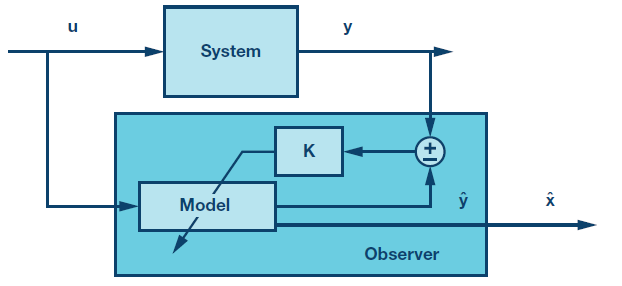
\includegraphics[width=0.5\textwidth]{Chap07/Figures/Kalman_principle.PNG}
    \caption{Kalman Filter Principle}
    \label{fig:Kalman_Filter_Principle}
\end{figure}

\section{Summer of the Chapter \ref{ch:Battery_SOC_Estimation_Algorithms}}
All over in chapter \ref{ch:Battery_SOC_Estimation_Algorithms}, I took an effort to gather focus on the Kalman approach to estimating the soc, is it only the algorithm in the literature well certainly not there are plenty of approaches are there in the literature to estimate the soc of the battery. Then a very obvious question is why Kalman's approach? Well, the answer is it is very immune to noise and accurate estimation, and it has proven most algorithms over decades. As an extension of this topic, we can use much more advanced approaches with Kalman, for instance, fuzzy networks with Kalman filter, support vector machines with Kalman, and many others... I have limited this chapter to 3 or 4 (Amper second, Kalman, EKF, UKF, AUKF) types of algorithms for soc estimation. Even we can look into machine learning, AI, and neural network approaches like the random forest, gradient descent, and stochastic gradient descent, etc. machine learning algorithms are more elegant and robust, but the drawback with those algorithms is we need a large amount of data to characterize the algorithms and tune, perhaps millions of data.  So it is not so easy to go ahead with the machine learning approach in smaller firms. Well, then Kalman's approach is the best among all? Not really it has drawbacks as well, but it holds sufficient grounds for estimating the battery soc.